\documentclass{beamer}

\usepackage{tikz}
\usetikzlibrary{calc}

\begin{document}

\begin{frame}[plain]

%\tikz[remember picture, overlay] \node[anchor=center] at (current page.center) {\includegraphics[width=0.2\textwidth]{foo}};

\begin{tikzpicture}[remember picture, overlay]
\node[anchor=center] at ($(current page.center) - (5cm,1cm)$) {\includegraphics[width=0.3\textwidth]{foo}};
\end{tikzpicture}


\begin{tikzpicture}[remember picture, overlay]
\node[anchor=center] at ($(current page.center) + (2.5cm,1.5cm)$) {\includegraphics[width=0.3\textwidth]{foo}};
\end{tikzpicture}

%\begin{tikzpicture}[remember picture,overlay]
  %\tikzset{shift={(current page.center)},yshift=0.0cm}
  %\tikzset{yshift=1.5cm}
  % the picture
%  \node[anchor=center] at (current page.center) {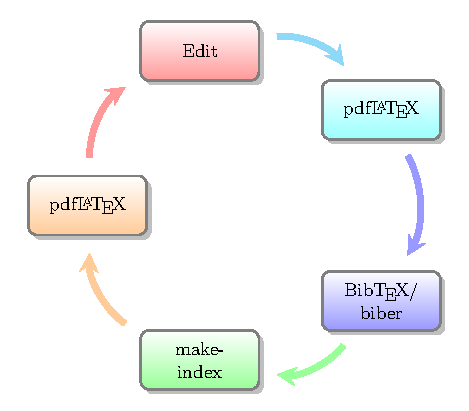
\includegraphics[width=0.5\textwidth]{../ex013/smart-circle.pdf}};
%\end{tikzpicture}


\end{frame}

\end{document}
